\documentclass[12pt,a4paper]{article}

% 如果需要中文支持,推荐使用xeCJK + 字体设置
\usepackage{xeCJK}
\setCJKmainfont{SimSun}  % 示例:宋体,可根据系统字体情况更换
\usepackage{amsmath}      % 数学公式(如有需要)
\usepackage{graphicx}     % 插图
\usepackage{geometry}     % 调整页边距
\usepackage{fancyhdr}     % 自定义页眉页脚
\usepackage{indentfirst}  % 中文首行缩进
\usepackage{calc}         % 允许做长度运算(测量文字宽度等)
\usepackage{titlesec}
\usepackage{booktabs} % 解决 \midrule 和 \bottomrule 报错
\usepackage{enumitem} % 支持自定义列表格式
\usepackage{graphicx}   % 处理图片
\usepackage{caption}    % 允许自定义 caption
\usepackage{subcaption} % 处理子图
\usepackage{float}      % 允许使用 [H] 选项,确保图片不浮动
\usepackage{multirow}

% 设置 \section 级标题为:加粗、大字号(如 \Large)
\titleformat{\section}
	{\bfseries\large}    % 标题自身的格式
	{\thesection}        % 标题编号的显示方式
	{1em}                % 编号与标题文字之间的间距
	{}                   % 在标题文字前后可插入额外代码,此处为空
	
% 设置 \subsection 级标题为:加粗、中等字号(如 \normalsize)
\titleformat{\subsection}
	{\bfseries\normalsize}
	{\thesubsection}
	{1em}
{}

% 页面设置(可根据需要微调)
\geometry{
	left=0.75cm,
	right=0.75cm,
	top=1cm,
	bottom=1.5cm
}

% 不需要过大的行距,使用较接近单倍行距的设置
\renewcommand{\baselinestretch}{1}

% 仅在页脚居中显示页码,页眉保持为空
\pagestyle{fancy}
\fancyhf{}  % 清空默认的页眉页脚
\fancyfoot[C]{\thepage}
\renewcommand{\headrulewidth}{0pt}
\renewcommand{\footrulewidth}{0pt}

% 首行缩进2字符(中文习惯)
\setlength{\parindent}{0pt}
\setlength{\leftskip}{2em}

\begin{document}
	%-------------------------------------------------------
	% 1 并排两个minipage:左标题、右校徽
	%   - 0.65\textwidth + 0.35\textwidth = \textwidth
	%   - 如果校徽过大或过小,可改宽度,如 0.25\textwidth、0.3\textwidth 等
	%   - 如果想让标题更大,可将 \Huge 改成 \huge 或 \LARGE
	%-------------------------------------------------------
	\noindent
	\hspace{-2em}
	\begin{minipage}[c]{0.65\textwidth}
		\raggedright
		{\fontsize{40pt}{60pt}\selectfont 物理实验报告}
	\end{minipage}
	\begin{minipage}[c]{0.35\textwidth}
		\raggedleft
		% 强制把校徽拉大到 0.35\textwidth 宽度 (高度自动匹配)
		% 若想指定高度,可用 "height=3cm" 等. 二选一即可.
		
\includegraphics[width=\linewidth, trim={20cm 20cm 20cm 20cm}, clip]{university_logo.png}
	\end{minipage}

	\vspace{-1em}
	

	%下方画两条分割线,并在两线之间写学号、姓名、日期、时间
	
	\hrule
	\vspace{0.4em}
	\noindent
	\begin{tabular}{l l l l}
    学号:\underline{114514} & 姓名:\underline{SUSTech} &
    日期:\underline{2025/03/18} & 时间:\underline{周二下午}
	\end{tabular}
	\vspace{-0em}
	\par
	\hrule

	
	\section{实验名称:透镜参数的测量及应用}
	
	\section{实验目的}
	了解光源、物、像间的关系,熟练掌握光具座上各种光学元件的共轴调节,并测量透镜的焦距。

	\section{实验仪器}
	光源,物屏,像屏,凸透镜,凹透镜,平面镜,光具座

	\section{实验原理}
		\subsection{高斯成像公式}
			在近轴条件近似下,高斯成像公式成立:
			\begin{equation}
			\frac{f^{\prime}}{p^{\prime}} + \frac{f}{p} = 1
			\end{equation}
			在空气中,有$f = -f^{\prime}$, \text{ 则高斯公式为:}
			\begin{equation}
			\frac{1}{p^{\prime}} - \frac{1}{p} = \frac{1}{f^{\prime}}
			\end{equation}
	
		\subsection{凸透镜焦距的测量}
			凸透镜焦距有多种方法,如:自准直法(平面镜反射法)、公式法、位移法
			\begin{figure}[H]
				\centering
				\begin{subfigure}{0.32\textwidth}
					\centering
					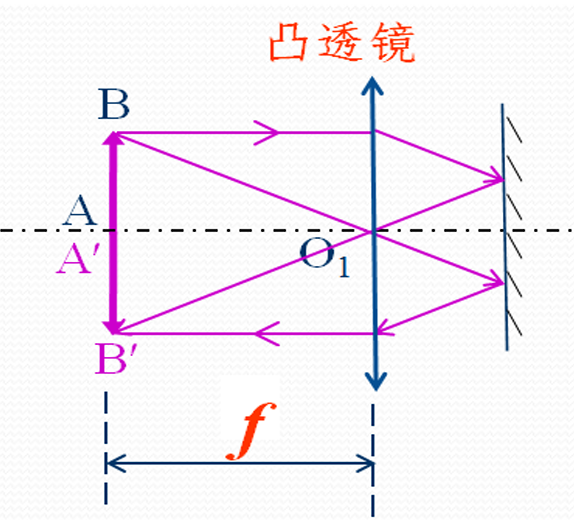
\includegraphics[width=0.8\textwidth]{自准直.png}
					\caption{自准直法(平面镜反射法)}
				\end{subfigure}
				\begin{subfigure}{0.32\textwidth}
					\centering
					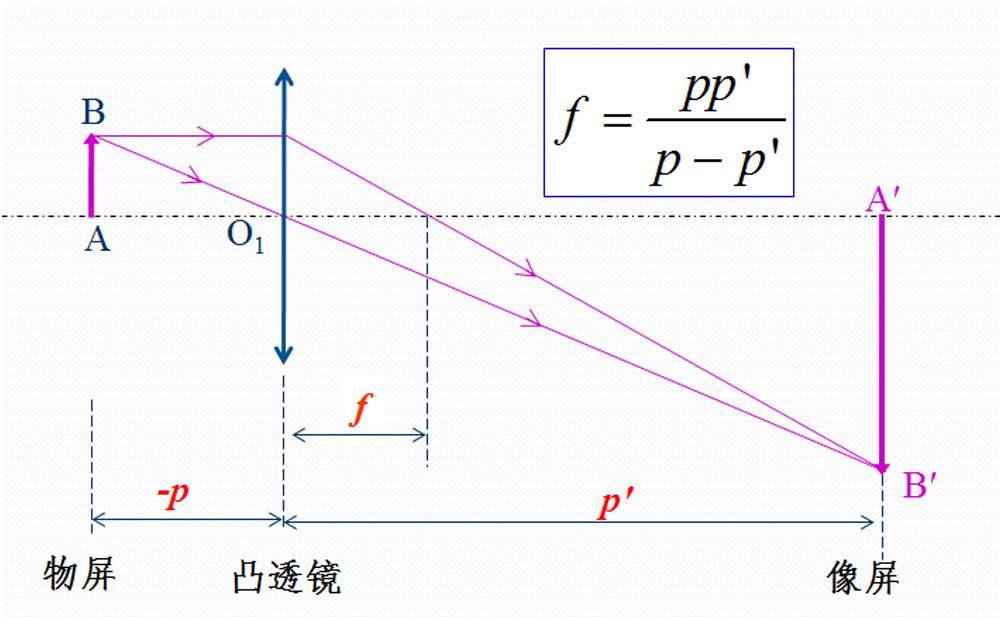
\includegraphics[width=\textwidth]{公式法.png}
					\caption{公式法}
				\end{subfigure}
				\begin{subfigure}{0.32\textwidth}
					\centering
					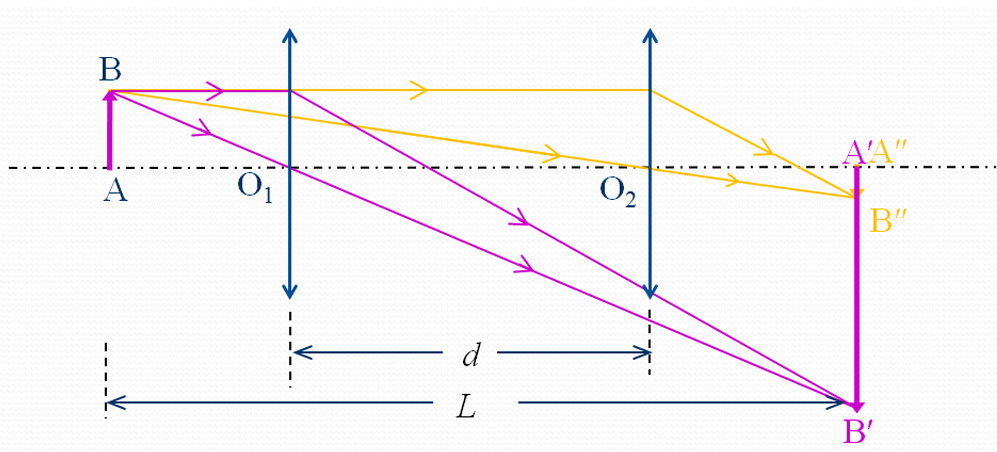
\includegraphics[width=1.2\textwidth]{位移法.png}
					\caption{位移法}
				\end{subfigure}
				\caption{光学示意图}
				\label{fig:formula_method}
			\end{figure}
			
			\subsubsection{自准直法(平面镜反射法)}
				如Figure 1.(a)自准直法(平面镜反射法),当平行光经过凸透镜后,其会在焦点处会聚。若在焦点处放置一个平面镜,则光线经镜面反射后,仍然通过凸透镜并变为平行光。调整透镜与平面镜的相对位置,使得入射光与反射光平行,则透镜到平面镜的距离即为焦距。
			\subsubsection{公式法}
				如Figure 1.(b)公式法,固定透镜,将物体放在距透镜一倍焦距以外的某处,在透镜的另一侧会形成一个清晰的实像。设 $p$ 和 $p^{\prime}$ 分别为物距和像距,即物体到透镜中心的距离和像到透镜中心的距离,根据高斯成像公式(\quad $\frac{1}{f} = \frac{1}{P} + \frac{1}{P^{\prime}}$ \quad) 可以计算透镜的焦距。
			\subsubsection{位移法}
				如Figure 1(c)位移法,对于一组固定的物距和像距(设总距离为 $D$),在物体与像屏之间移动透镜,找到两个可以形成清晰像的位置,分别记为 $u_1$ 和 $u_2$。设透镜的位移距离为 $d$,则透镜焦距可由以下公式计算:
				\begin{equation}
			 	f = \frac{D^2 - d^2}{4D}
				\end{equation}

		\subsection{凹透镜焦距的测量——辅助透镜法}
			\begin{figure}[htbp]
			\centering
			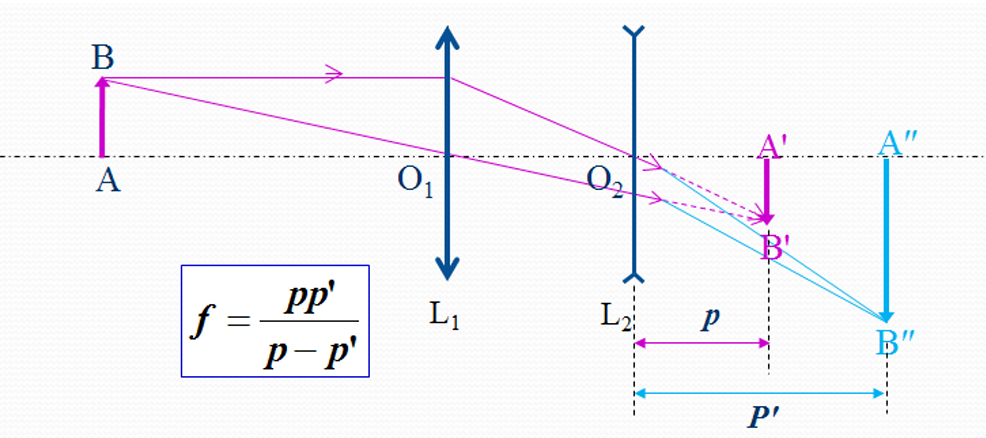
\includegraphics[width=0.49\textwidth]{辅助透镜法1.png}
			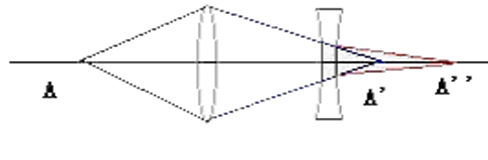
\includegraphics[width=0.49\textwidth]{辅助透镜法2.png}
			\caption{辅助透镜法}
			\label{fig:chart1}
		\end{figure}
	
			如Figure 2.辅助透镜法,凹透镜是发散透镜,正常仅成虚像。为测量像距,可利用凸透镜成的像作为凹透镜的物,再成一个实像。
			计算公式如图:
			\begin{equation}
				f=\frac{pp^\prime}{p-p^\prime}
			\end{equation}
		
	\section{实验内容}

	\subsection{光学元件的共轭调整}
	\paragraph{调整要求} 
	1)所有光学器件的光轴重合 \quad 2)所有的光轴与光具座的导轨平行
	\paragraph{粗调}
		将光学元件较紧凑地放置在光具座上,用眼睛观察调节,使光学元件中心处在与导轨平行的同一直线,同时各元件相互平行且垂直光具座
	\paragraph{细调}
	    利用二次成像法调节,当两次成像中心完全重合时表示各光学元件共轴
	
	\subsection{测量凸透镜的焦距}
	使用上述 \, 自准直法、公式法、位移法 \, 测量凸透镜焦距。记录多组测量数据,每组数据测量五次,并对结果进行误差分析,比较三种方法的测量结果。
	
	\subsection{测量凹透镜的焦距}
		采用辅助透镜法测量凹透镜焦距:测量组合透镜焦距 $f$,结合单独测量的凸透镜焦距 $f_1$,计算凹透镜焦距 $f_2$。记录数据并进行误差分析。


	\section{数据记录}
	见附件及7.数据处理

	\section{数据处理}
		\subsection{凸透镜焦距}	
			\subsubsection{自准直法(平面镜反射法)}
				\begin{table}[h]
				\centering
				\renewcommand{\arraystretch}{1.2}
				\begin{tabular}{|c|c|c|}
					\hline
					自准直法 & 物屏位置$x_0$/cm & 像屏位置$x_1$/cm \\
					\hline
					1 & \multirow{4}{*}{12.00} & 27.01 \\
					\cline{1-1} \cline{3-3}
					2 &  & 26.92 \\
					\cline{1-1} \cline{3-3}
					3 &  & 26.80 \\
					\cline{1-1} \cline{3-3}
					平均 &  & 26.91 \\
					\hline
					焦距 $f$/cm & \multicolumn{2}{c|}{14.91} \\
					\hline
				\end{tabular}
				\caption{自准直法实验数据及计算结果}
				\end{table}
				通过实验数据及自准直法焦距计算公式,计算出
				$f=\overline{x_{1}}-\overline{x_{0}}=26.91-12.00=14.91cm$
				
			\subsubsection{公式法}
				\begin{table}[h]
					\centering
					\renewcommand{\arraystretch}{1.2}
					\begin{tabular}{|c|c|c|c|}
						\hline
						公式法 & 物屏$x_0$/cm & 透镜 $x_1$/cm & 像屏 $x_2$/cm \\
						\hline
						1 & \multirow{4}{*}{12.00} & \multirow{4}{*}{43.00} & 72.55 \\
						\cline{1-1} \cline{4-4}
						2 &  &  & 71.13 \\
						\cline{1-1} \cline{4-4}
						3 &  &  & 71.93 \\
						\cline{1-1} \cline{4-4}
						平均 &  &  & 71.87 \\
						\hline
						焦距 $f$/cm & \multicolumn{3}{c|}{14.95} \\
						\hline
					\end{tabular}
					\caption{公式法实验数据及计算结果}
				\end{table}
				通过实验数据及公式法焦距计算公式,计算出
				$f=\frac{\overline{p}\overline{p}}{\overline{p}-\overline{p}^{\prime}}=\frac{(71.87-43.00)\times (12.00-43.00) }{(12.00-43.00)-(71.87-43.00)} \approx 14.95cm$
				
			\subsubsection{位移法}
				\begin{table}[h]
				\centering
				\renewcommand{\arraystretch}{1.2}
				\begin{tabular}{|c|c|c|c|c|}
					\hline
					位置法 & 物屏 $x_0$/cm & 透镜 $x_1$/cm & 透镜 $x_2$/cm & 像屏 $x_3$/cm \\
					\hline
					1 & \multirow{4}{*}{12.00} & 31.58 & 72.10 & \multirow{4}{*}{92.00} \\
					\cline{1-1} \cline{3-4}
					2 &  & 31.78 & 72.31 &  \\
					\cline{1-1} \cline{3-4}
					3 &  & 31.62 & 71.85 &  \\
					\cline{1-1} \cline{3-4}
					平均 &  & 31.66 & 72.09 &  \\
					\hline
					焦距 $f$/cm & \multicolumn{4}{c|}{14.89} \\
					\hline
				\end{tabular}
				\caption{位移法实验数据及计算结果}
			\end{table}
			通过实验数据及位移法焦距计算公式,计算出
			$f = \frac{D^2 - d^2}{4D} = \frac{(\bar{x}_{3}-\bar{x}_{0})^{2}-(\bar{x}_{2}-\bar{x}_{1})^{3}}{4(\bar{x}_{3}-\bar{x}_{0})} = \frac{(92.00-12.00)^2-(72.09-31.66)^2}{4 \times (92.00-12.00)} \approx 14.89cm$

		\subsection{凹透镜焦距}	
			\begin{table}[H]
			\centering
			\renewcommand{\arraystretch}{1.2}
			\begin{tabular}{|c|c|c|c|c|}
				\hline
				辅助透镜法 & 凸透镜位置/cm & 凸透镜成像$x_0$/cm & 凹透镜位置$x_1$/cm & 像屏$x_2$/cm \\
				\hline
				1 & \multirow{4}{*}{72.00} & 92.10 & 88.25 & \multirow{4}{*}{98.80} \\
				\cline{1-1} \cline{3-4}
				2 &  & 92.25 & 88.43 &  \\
				\cline{1-1} \cline{3-4}
				3 &  & 92.00 & 88.14 &  \\
				\cline{1-1} \cline{3-4}
				平均 &  & 92.12 & 88.27 &  \\
				\hline
				焦距 $f$/cm & \multicolumn{4}{c|}{-6.07} \\
				\hline
			\end{tabular}
			\caption{辅助透镜法实验数据及计算结果}
			\end{table}
			通过实验数据及辅助透镜法焦距计算公式,计算出
			$f=\frac{\overline{p}\overline{p}}{\overline{p}-\overline{p}^{\prime}}=\frac{(\overline{x}_{2}-\overline{x}_{1})(\overline{x}_{3}-\overline{x}_{1})}{(\overline{x}_{3}-\overline{x}_{2})} \approx -6.07cm$

		\subsection{误差分析}
		由凸透镜标准焦距为15.00cm,凹透镜标准焦距为-6.00cm可得误差百分比的结果如下:\\
		自准直法为 $0.6\%$ \quad 公式法为 $0.03\%$ \quad 位移法为 $0.73\%$ \quad 辅助透镜法为 $1.17\%$。\\
		实验中可能导致误差的主要因素包括:
			\begin{itemize}
				\item \textbf{仪器精度}:设备的测量精度不足,例如标尺的最小刻度、光学装置的对准误差等。
				\item \textbf{环境条件}:如光照等环境因素的变化可能影响实验结果。
				\item \textbf{实验操作}:实验者在操作中对图像位置一定存在主观判断,导致数据记录不准确等。
			\end{itemize}


	\section{问题思考}
		\paragraph{自准直法} 该方法依赖平面镜反射成像的对焦判断,需通过调整透镜位置使物屏上的像清晰。由于人眼对成像清晰度的主观判断存在差异且物屏与像屏的位置测量可能存在微小偏差,导致误差适中。
		\paragraph{公式法}   由于公式法操作简单,且测量像屏位置误差可能可部分与测量透镜位置误差抵消,导致误差最小。
		\paragraph{位移法}   理论误差应最小。但实际由于步骤麻烦,操作难度较大,测量数据较多,误差累积,以及平方项对误差敏感,致使误差最大。
	
	\section{实验结论}
	\begin{table}[h]
		\centering
		\renewcommand{\arraystretch}{1.2}  % 可根据需要调整行高
		\begin{tabular}{|c|c|c|c|c|}
		\hline
		\textbf{透镜种类} & \textbf{焦距理论值/cm} & \textbf{实验方法} & \textbf{测量实际值/cm} & \textbf{误差百分比} \\
		\hline
		\multirow{3}{*}{凸透镜} & \multirow{3}{*}{15.00} & 自准直法 & 14.91 & 0.60\% \\
		\cline{3-5}
		 &  & 公式法 & 14.95 & 0.03\% \\
		\cline{3-5}
		 &  & 位移法 & 14.89 & 0.73\% \\
		\hline
		凹透镜 & -6.00 & 辅助透镜法 & -6.07 & 1.17\% \\
		\hline
		\end{tabular}
		\caption{实验结果}
		\label{tab:lens-data}
		\end{table}


\end{document}
